% Chapter 3

\chapter{Related Work} % Main chapter title

\label{Related Work} % For referencing the chapter elsewhere, use \ref{Chapter1} 

\lhead{Chapter 3. \emph{Related Work}} % This is for the header on each page - perhaps a shortened title

This chapter presents related research work in evolutionary methodologies used to evolve robot controllers as well as robot morphologies in simulated or physical environments. In addition a lot of research work has been conducted regarding the aspect of the evolution in soft-robots. With the designing freedom soft materials give to any evolutionary method it is of interest to see what has been achieved so far. Novelty search as discussed in section~\ref{NoveltySearch}, is a diversity based method, where the objective function rewards the novelty in the behavior level. As it will be discussed later in this chapter, novelty search has been used within a evolutionary setting in order to evolve virtual creatures.


\section{Evolution of Virtual-Physical Robots}

Robot controllers can be evolved through evolutionary algorithms on simulated (virtual) robots. Moreover, evolutionary methods can be applied to physical~robots~\citep{nolfi1994evolve} as well, where no damage can occur due to exploration of the action space. Controllers represented by an encoding scheme can be generated and propagated from generation to generation within an evolutionary framework, until good solutions will be found.

\begin{figure}[b!]
\centering
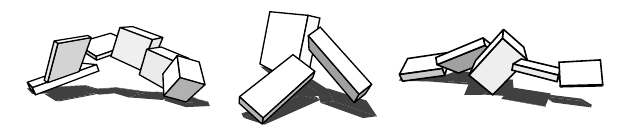
\includegraphics[width=0.8\textwidth]{../Figures/Misc/evolvingVirtualCreatures.png}
\caption{Karl Sims, ``evolution of virtual creatures'' \citep{sims1994evolving}.}
\label{fig:karlSims}
\end{figure}

Novel systems, that make use of evolutionary methods to evolve complex encoding representations such as artificial neural networks have been developed. These complex representations can control not only the morphology of rigid body parts connected with joints, but also control the forces applied to each joint. As a result, virtual creatures (see Fig.~\ref{fig:karlSims}) can be produced~\citep{sims1994evolving} in a physical three dimensional world. Different fitness measures also give the possibility of the evolution of diverse creatures in respect to these measures. This genetic encoding defines a hyperspace of infinite number of possible creatures and behaviors, and when it is searched using optimization techniques like EA, a variety of successful and interesting locomotion strategies emerge, some of which would be difficult to invent or build by engineers. This was the first work successfully tried to evolve both the morphology and the locomotion of virtual robots in a simulated environment, based on such a complex representation for the genome (ANNs).

\begin{figure}[t!]
\centering
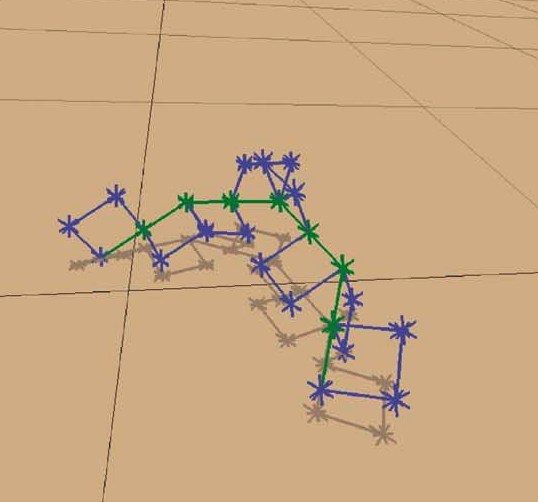
\includegraphics[width=0.25\textwidth,height=0.2\textwidth]{../Figures/Misc/lsystems1.png}
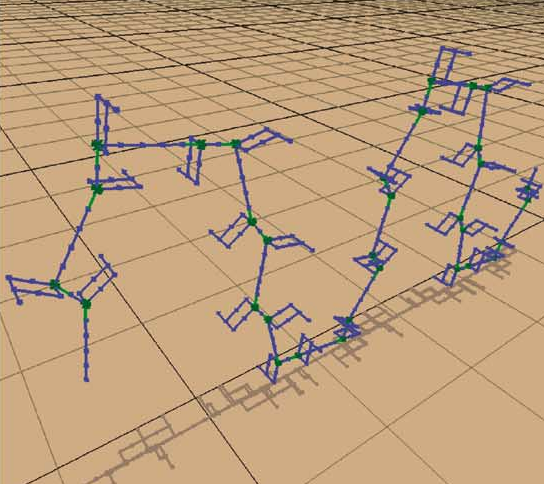
\includegraphics[width=0.25\textwidth,height=0.2\textwidth]{../Figures/Misc/lsystems2.png}
\caption{The use of Lindenmayer systems results in creature morphologies that have a more natural look~\citep{hornby2001evolving}.}
\label{fig:lsystems}
\end{figure}

Computer graphic designers can profit from evolutionary techniques, since the design phase of some applications (i.e games, movies, etc.) is a time consuming process. However, the need for natural looking morphologies is of crucial importance. Previous work~\citep{lipson2000automatic,sims1994evolving} resulted in unnatural looking shapes for the evolving virtual creatures and abnormal behaviors mostly due to vast solution space, and the encoding representation of the genome. A system that uses Lindenmayer systems~\citep{hornby2001evolving} (L-systems) as the encoding of an EA for creating virtual creatures. Creatures evolved by this system have hundreds of parts, and the use of an L-system as the encoding resulted in creature morphologies that have a more natural look (see Fig.~\ref{fig:lsystems}). Thus, this work~\citep{hornby2001evolving} showed that the encoding of the genome can indeed have a big impact on the evolved morphologies.

\begin{figure}[h!]
\centering
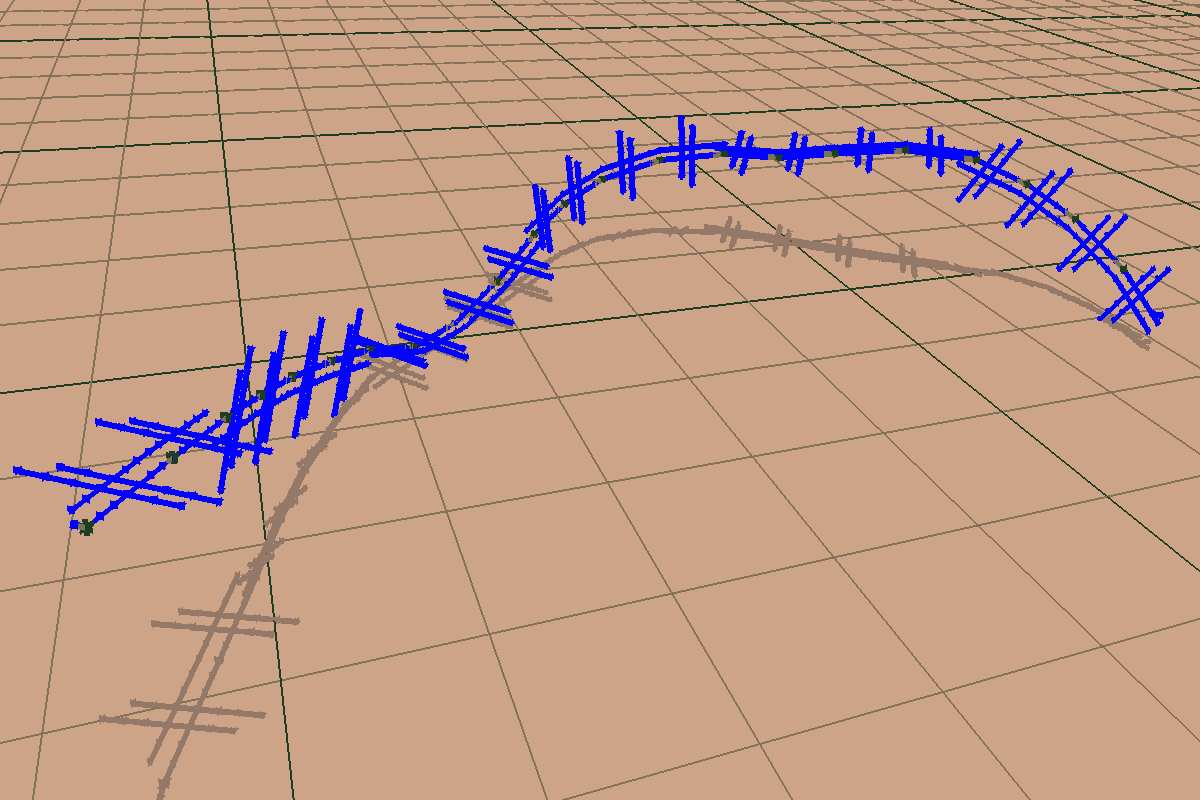
\includegraphics[width=0.25\textwidth,height=0.2\textwidth]{../Figures/Misc/rules1.png}
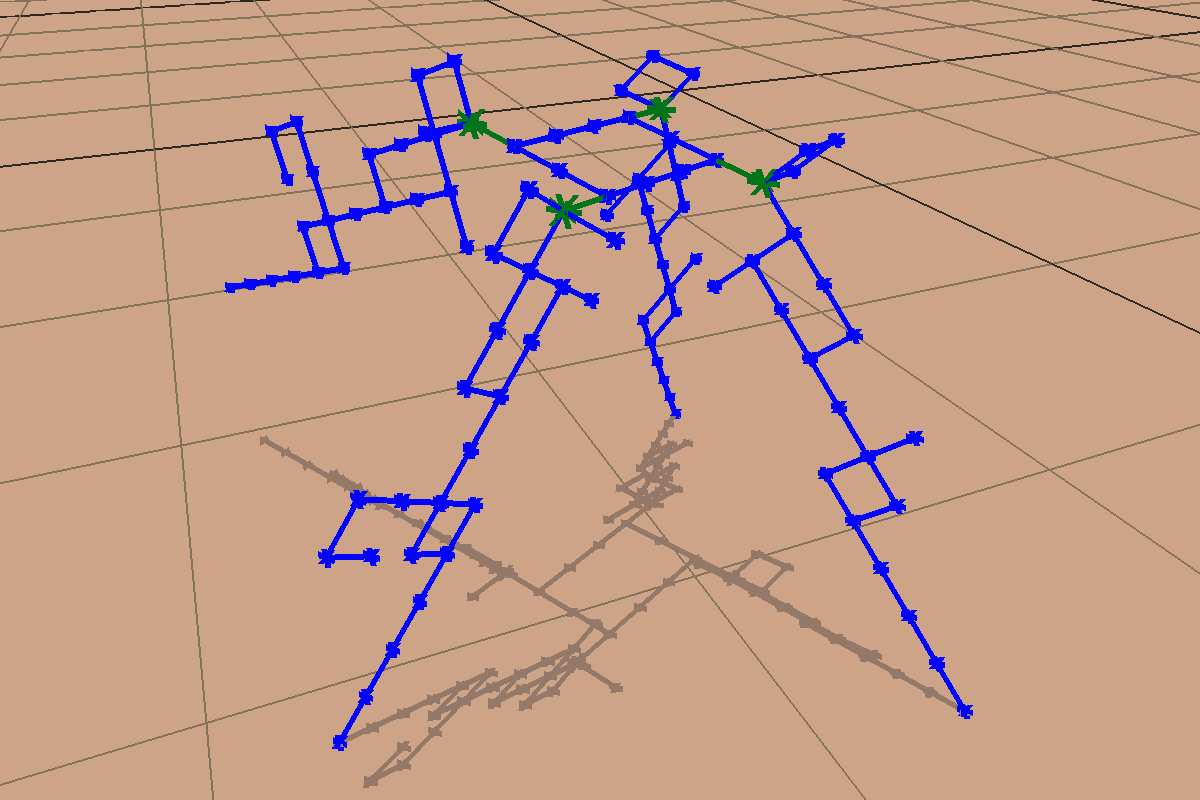
\includegraphics[width=0.25\textwidth,height=0.2\textwidth]{../Figures/Misc/rules2.png}
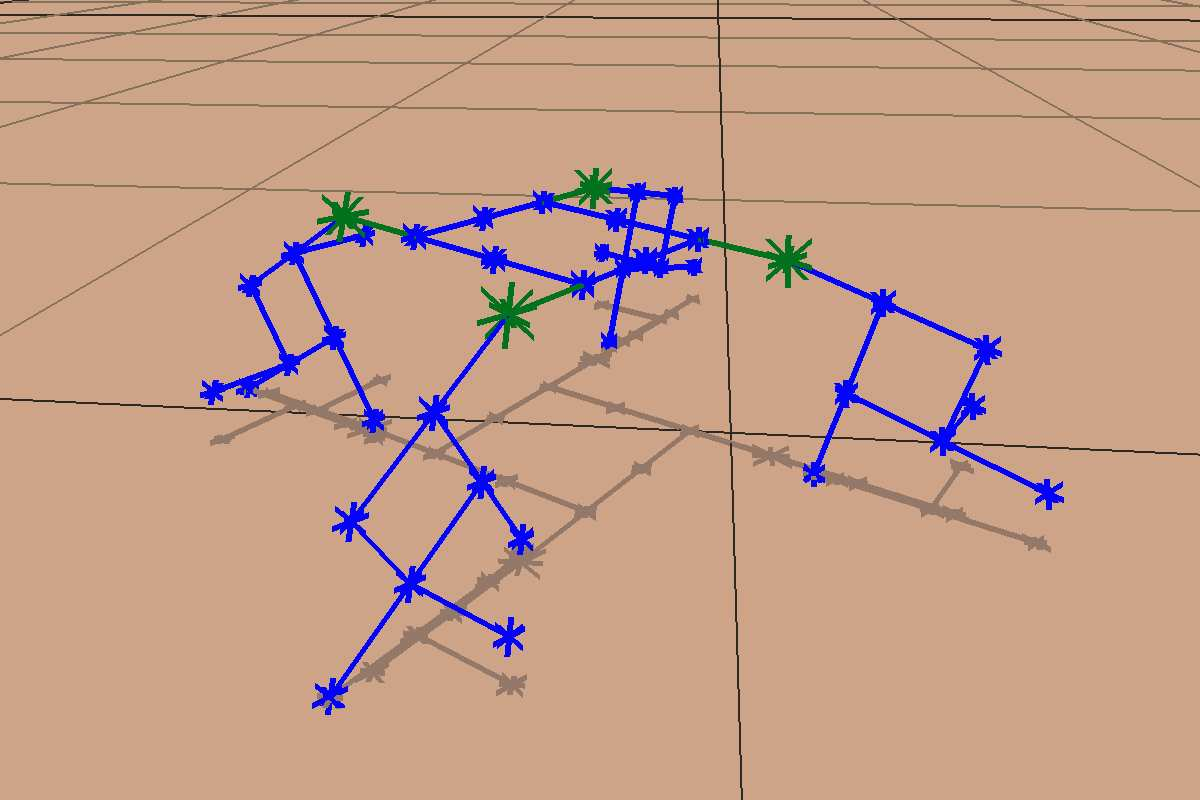
\includegraphics[width=0.25\textwidth,height=0.2\textwidth]{../Figures/Misc/rules3.png}
\caption{Generative representation can define a set of rules that simple components can be put together to generate a robot~\citep{hornby2003generative}.}
\label{fig:rules}
\end{figure}

Evolutionary robotics have shown the ability to evolve complex designs which can perform tasks in the environment, they are evolved in. However, these complex designs are hard or sometimes impossible to be transferred on a physical robot. Generative representation used in~\citep{hornby2003generative}, accomplishes to replace complex representations into a construction plan which uses simple robot components in a regular way (see Fig.~\ref{fig:rules}). This compact design space of the resulted method, can indeed limit the possible morphologies given a set of possible morphological parts. As direct encoding schemes have trouble capturing geometrical properties of the problem, generative encoding like CPPNs can be used in order to take advantage of a problem's regularities and symmetries.

\begin{figure}[t!]
\centering
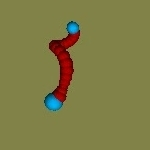
\includegraphics[width=0.25\textwidth,height=0.2\textwidth]{../Figures/Misc/auerbach1.png}
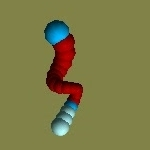
\includegraphics[width=0.25\textwidth,height=0.2\textwidth]{../Figures/Misc/auerbach2.png}
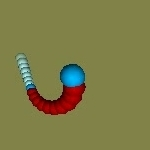
\includegraphics[width=0.25\textwidth,height=0.2\textwidth]{../Figures/Misc/auerbach3.png}
\caption{CPPN-NEAT can be used as a generative encoding for the evolution of virtual robots~\citep{auerbach2010dynamic}.}
\label{fig:auerbach}
\end{figure}

HyperNEAT~\citep{stanley2009hypercube}, which is a method to evolve CPPNs which will determine the topology and the weights of ANNs, shows promising results in evolving the gaits of legged robots~\citep{clune2009evolving}, where direct encodings have trouble. Natural evolution is the only process which instead that evolving only the brain of biological organisms, it also evolves the morphologies of them. CPPN-NEAT~\citep{stanley2007compositional} can be used as a generative encoding EA which can evolve both features of virtual robots~\citep{auerbach2010dynamic, auerbach2010evolving} (see Fig.~\ref{fig:auerbach}), implying that more complex creatures than designers imagination can be created in such a setting. It is also possible that a lower resolution is used at the first runs of the evolution to save computational time without significantly degrading the quality of evolved structures and later a higher resolution for the details optimization.

It has also been shown that evolving objects with types of encoding based on concepts from biological development like CPPN can be a powerful way to evolve complex, interesting objects~\citep{clune2011evolving}. These results can be used in applications in fields of engineering, biology, and as diverse as art. Apart from the use in robot-bodies design evolution, EA techniques coupled with indirect coding schemes allow the evolution of the morphology and the motion control of soft bodies, in this case  multicellular animats~\citep{joachimczak2012co} in a 2-dimensional fluid-like environment. Both the developmental program and motion control are encoded indirectly in a single linear genome, where a genetic algorithm can be applied to evolve it.

With the excel of $3$D printing, soft multi-material robot bodies can actually be produced using simple material types. These soft structures made only by soft materials can be simulated~\citep{hiller2012dynamic} allowing for the evolution of their design without the costs of production. As it is first shown in~\citep{hiller2012automatic}, the automated design of three dimensional bodies which can obtain functionalities through the distribution of hard and soft materials inside the three dimensional space. The robots were evolved (EA) and tested for a single-direction locomotion displacement, whereas it has also been proved, testing a soft material robot inside a pressure-chamber that, the actual error compared to the virtual one in the simulation was small.

\begin{figure}[t!]
\centering
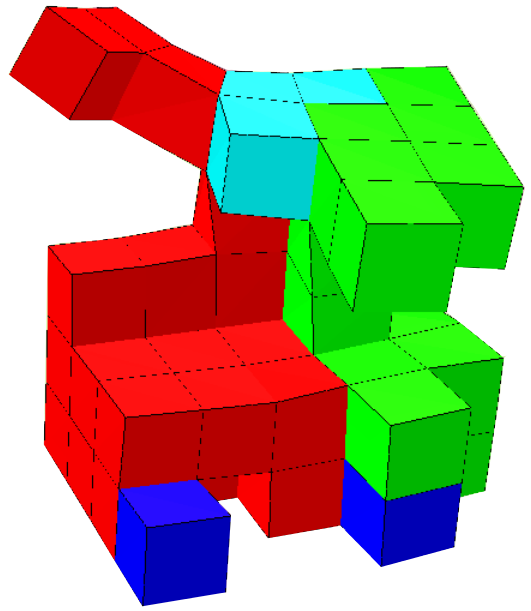
\includegraphics[height=0.2\textwidth]{../Figures/Misc/unshacklingEvolutionFigure1.png}\hspace{0.4cm}
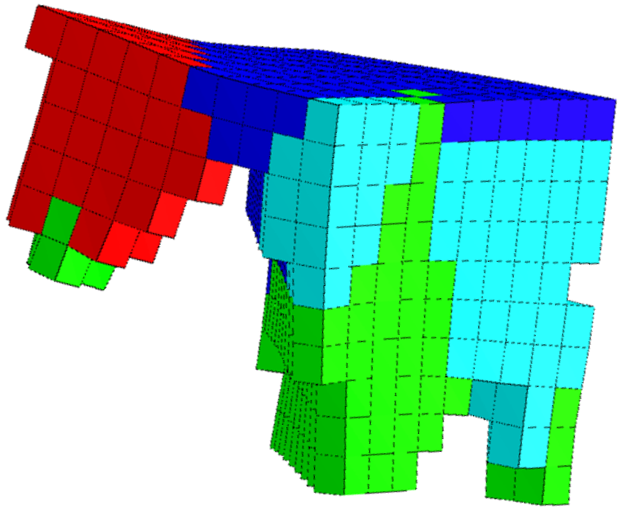
\includegraphics[height=0.2\textwidth]{../Figures/Misc/unshacklingEvolutionFigure2.png}\hspace{0.4cm}
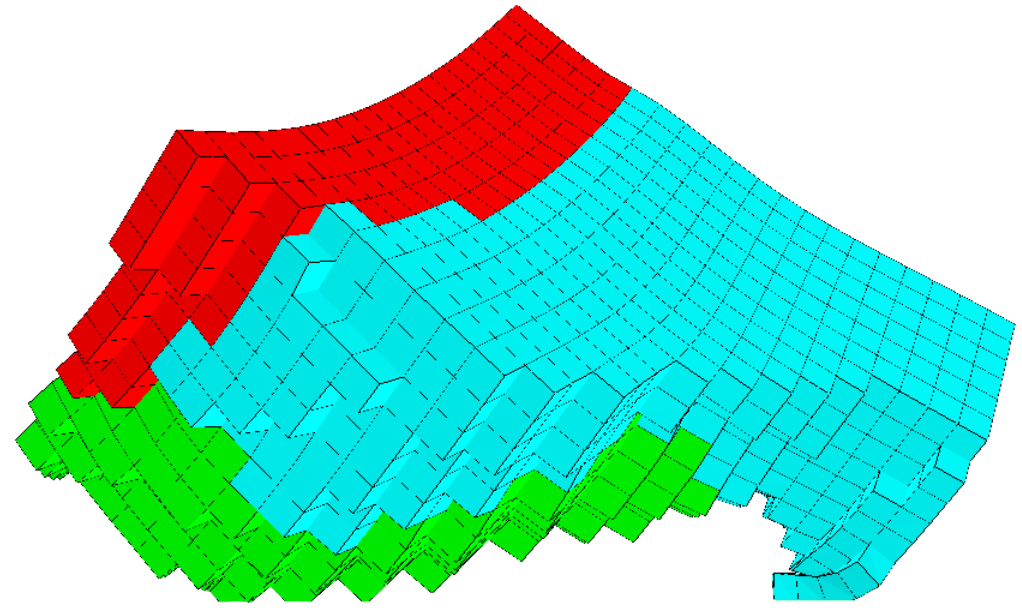
\includegraphics[height=0.2\textwidth]{../Figures/Misc/unshacklingEvolutionFigure3.png}
\caption{Evolution of soft robots' morphology by indirect encoding (CPPN) \citep{cheney2013unshackling}.}
\label{fig:unschackling}
\end{figure}


\begin{figure}[b!]
\centering
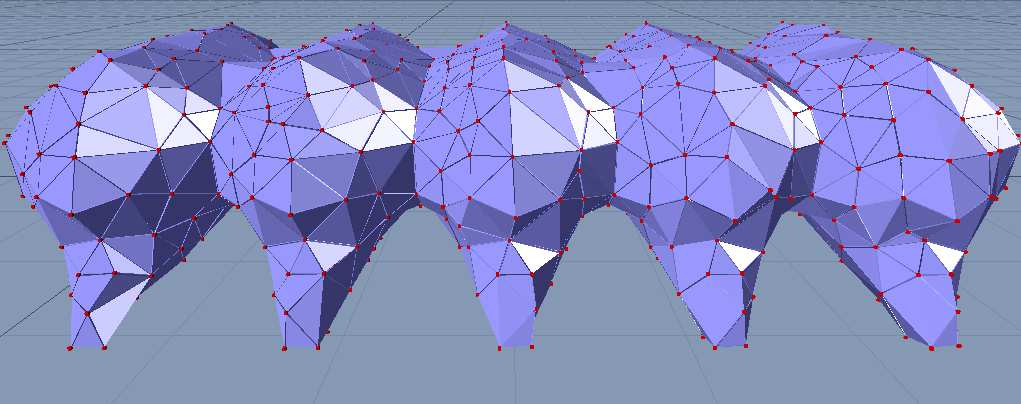
\includegraphics[width=0.6\textwidth]{../Figures/Misc/meshSoft1.png}
\caption{Soft bodies are built out of meshes of tetrahedra in~\citep{rieffel2014growing}.}
\label{fig:meshSoft}
\end{figure}

Evolution of soft material robots as was also shown in~\citep{hiller2012automatic} can produce structures able to locomote. The possibility of evolving these soft structures using indirect coding was of interest to be exploited by~\citep{cheney2013unshackling}. A powerful generative encoding, CPPN~\citep{stanley2007compositional}, used to generate soft voxel-formed three dimensional structures (see Fig.~\ref{fig:unschackling}) like in~\citep{hiller2012automatic}, coupled with the use of NEAT algorithm which ensures the increase of complexity of the networks produced, were purposed for evolving these soft-robots. The superiority of this kind of generative encoding was verified, showing how CPPNs can take advantage of the geometrical properties they show. Evaluation was done by a simple displacement measure. Yet, evolution tended to stick to different kinds of locomotion strategies and morphologies as the fitness function was penalized for different kinds of parameters. Furthermore, it has been shown that evolving morphologies (CPPNs) in lower resolutions and then applying the same networks for higher resolution structures can be beneficial, since the locomotion behaviors in lowers structures apply also in higher, saving in this way computational time.  An earlier work~\citep{hiller2010evolving}, apart from the generative encoding of CPPNs, used \textit{Gaussian Mixture} and \textit{Discrete Cosine Transform} to produce amorphous soft-body structures.

The simultaneous evolution of soft-robot morphology and control was also investigated by recent work~\citep{rieffel2014growing} (see Fig.~\ref{fig:meshSoft}). Some aspects of soft-robot evolution were verified in this work, namely muscle placement and muscle-firing patterns can be evolved given a fixed body shape and fixed material properties. Furthermore, material properties can be co-evolved alongside locomotion strategies. Finally, a developmental encoding was introduced, allowing more complex parts to be added to soft-robotic structures during the evolution.


\section{Evolving Virtual Creatures by Novelty Search}

\begin{figure}[t!]
\centering
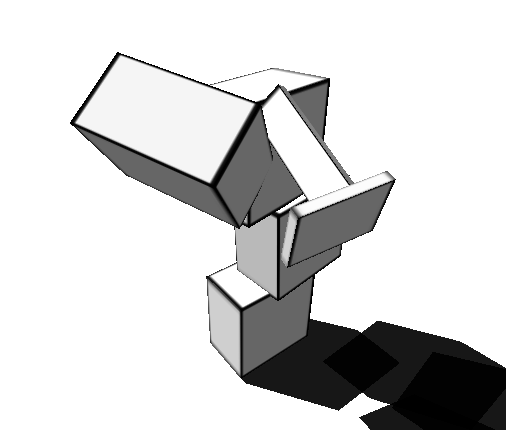
\includegraphics[width=0.2\textwidth]{../Figures/Misc/nov1.png}
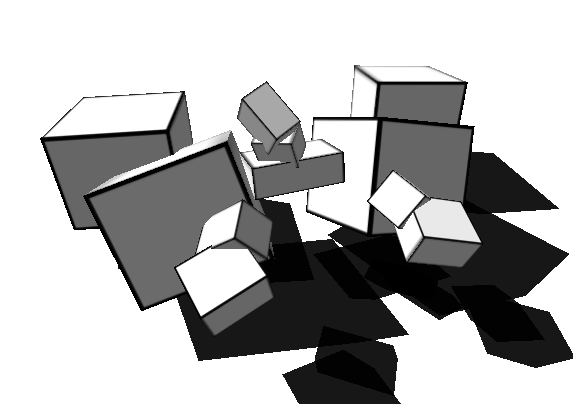
\includegraphics[width=0.2\textwidth]{../Figures/Misc/nov2.png}
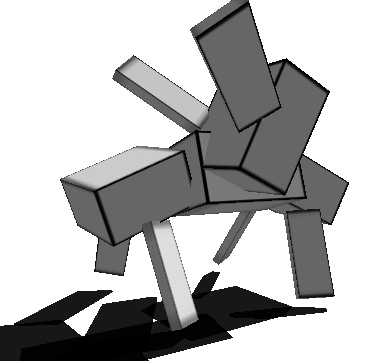
\includegraphics[width=0.2\textwidth]{../Figures/Misc/nov3.png}
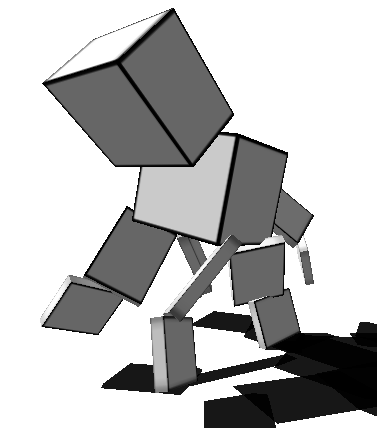
\includegraphics[width=0.2\textwidth]{../Figures/Misc/nov4.png}
\caption{Diverse morphologies evolved during a single run of novelty search with local competition~\citep{lehman2011evolving}.}
\label{fig:noveltySims}
\end{figure}

In problem with such high dimensionality as evolving both the morphology and locomotion strategy of artificial creature in simulated or physical environments, evolution does not explore the solution space enough, sticking only with first easiest to exploit morphologies. However, novelty search, a technique that explicitly rewards diverging, can potentially mitigate such convergence. Methods for evolving such virtual creatures like in~\citep{sims1994evolving}, can utilize novelty search~\citep{lehman2011evolving}, and be far more explorative in the search space (see Fig.~\ref{fig:noveltySims}). Behavior novelty defined as a measure between morphological properties of the produced creatures driving the evolution to explore more diverse morphologies. This kind of defined behavior cannot led the larger diversity of creatures to move, as different produced morphologies does not guarantee that some of them will actually move. However, combining fitness and novelty metrics through local competition led to improved results, whereas novelty search alone failed. 



\begin{comment}
\section{Evolving gaits}
\todo{Not much idea of what to add here and where I should focus (space?)}
\citep{auerbach2012relationship} On  the  relationship  between  environmental and mechanical complexity in evolved robots.
\citep{lee2013evolving} Evolving gaits  for  physical  robots  with  the  hyperneat  generative  encoding:   The  benefits  of simulation.
\end{comment}
